\documentclass[12pt]{beamer}
\usepackage{beamerthemeHannover, graphicx, clrscode, amsmath, amssymb, multicol}
\usepackage{verbatim}
\setbeamercolor{sidebar}{use=structure,bg=gray!20!red!60!white}
\title{Blizkost \\ \small{ A bridge between Perl 5 and Perl 6 } }
\author[Duke Leto]{Jonathan "Duke" Leto}
\date{}

\begin{document}

\frame{
    \titlepage
    \begin{center}
    %    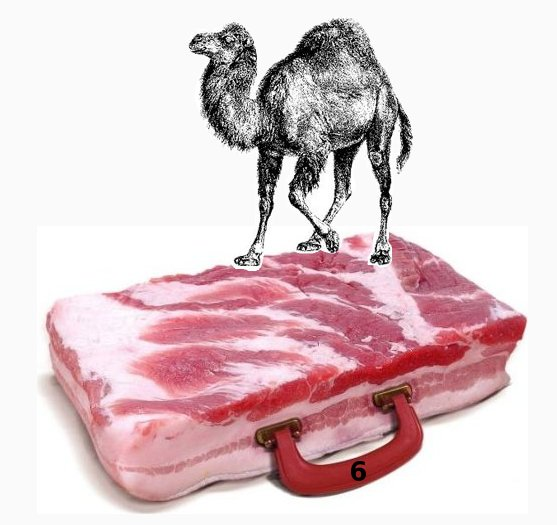
\includegraphics[width=4.57cm, height=4.25cm]{perl6bacon}
    \end{center}
}

\section{What is Blizkost?}
\frame{
    \frametitle{Flavors of Perl 6}
    \begin{center}
        \begin{itemize}
            \item Rakudo - Parrot
            \item Pugs - Haskell
            \item SMOP - C+DSLs
            \item Elf - Ruby
            \item STD.pm - Larry's Implementation in Perl 6 (gimme5)
            \item v6.pm - Source filter for Perl 5
            \item others ...
        \end{itemize}
    \end{center}
}


\frame{
    \frametitle{ Thanks }
    \begin{itemize}
        \item Larry
        \item Eric Wilhelm
        \item Jerry Gay
        \item Patrick Michaud
        \item The Perl Foundation
        \item Everyone working on Parrot, Rakudo and Perl 6
    \end{itemize}
}

\frame{
    \frametitle{ Resources }
    \begin{center}
        \begin{itemize}
           \item http://rakudo.org
           \item http://parrot.org
           \item http://perlsphere.net
           \item \#perl6 and \#parrot on freenode
           \item \#pdx.pm on irc.perl.org
        \end{itemize}
    \end{center}
}
\end{document}
